\documentclass[letterpaper,10pt]{article}
\usepackage{graphicx}
\usepackage{listings}
\usepackage{fullpage}
\usepackage{fixltx2e}
\usepackage{multirow}
\usepackage{amssymb,amsmath}
\usepackage{mathtools}
\usepackage{bm}
\usepackage[hyperfootnotes=false]{hyperref}
\usepackage{url}
\usepackage{subfig}
\usepackage{relsize}
\usepackage{enumitem}
\usepackage{fancyhdr}
\usepackage{framed}
\setlength{\headheight}{14pt}
\pagestyle{fancy}
\headsep = 20pt

% Lineskip mods
\linespread{1.0}
\setlength{\parskip}{0.5\baselineskip}
\setlength{\parindent}{0pt}
\newlength\docparskip
\parskip=6pt
\setlength{\docparskip}{\parskip}
\renewcommand{\arraystretch}{1.085}
\usepackage{xcolor}
\lstset{basicstyle=\ttfamily,
  showstringspaces=false,
  commentstyle=\color{red},
  keywordstyle=\color{blue}
}
\begin{document}

\fancyhf{}
\fancyhead[L]{AME 60614: Numerical Methods}
\fancyhead[R]{Qihao Zhuo: Problem Set 3}
\fancyfoot[C]{\thepage}

\thispagestyle{plain}
\begin{center}
  \large
  \textbf{AME 60614: Numerical Methods} \\
  \textbf{Fall 2021} \\
  \vspace{0.5em}
  \textbf{Problem Set 3} \\
  \vspace{1em}
  Qihao Zhuo
\end{center}

\vspace{1.5em}

\section{Iteratively Implicit Methods}\label{sec1}
\subsection{a}
\begin{align}
  y^*_{n+1}&=y_n+hf+O(h^2)\notag\\
  y_{n+1}&=y_n+\frac{h}{2}\left(f^*_{n+1}+f\right)\notag\\
  &=y_n+\frac{h}{2}\left(f+f+hf_t+hff_y+O(h^2)\right)\notag\\
  &=y_n+hf+\frac{h^2}{2}f_t+\frac{h^2}{2}ff_y+O(h^3)\label{eq1_1_1}
\end{align}

With Taylor Expansion, 
\begin{equation}
  y_{n+1}=y_n+hf+\frac{h^2}{2}f_t+O(h^3)\label{eq1_1_2}
\end{equation}

Comparing Eq.~\ref{eq1_1_1} and Eq.~\ref{eq1_1_2}, the $\frac{h^2}{2}ff_y$ term cannot eliminate so the order of accuracy after the first corrector step is $O(h^2)$. 
%\begin{align*}
%  y^2_{n+1}&=y_n+hf+\frac{h^2}{2}f_t+\frac{h^2}{2}ff_y+O(h^3)\\
%  y^3_{n+1}&=y_n+\frac{h}{2}\left(f^2_{n+1}+f\right)\\
%  f^2_{n+1}&=f+hf_t+\left(hf+\frac{h^2}{2}f_t+\frac{h^2}{2}ff_y\right)f_y\\
%  y^3_{n+1}&=y_n+\frac{h}{2}\left(f^2_{n+1}+f\right)\\
%  &=y_n+\frac{h}{2}\left[f+hf_t+\left(hf+\frac{h^2}{2}f_t+\frac{h^2}{2}ff_y\right)f_y+f\right]\\
%  &=y_n+hf+\frac{h^2}{2}f_t+\frac{h^2}{2}ff_y+\frac{h^3}{4}f_tf_y+\frac{h^3}{4}ff_y^2
%\end{align*}

From an accuracy standpoint, there is always shift in $y$. So with more corrector steps, the accuracy could not be raised to $O(h^3)$. And when $h$ is small enough, the $y^*_{n+1}$ 
will be a close predictor, which makes addtional corrector unnecessary. 

\subsection{b}
For ABM1, 
\begin{align*}
  y^{'}&=f(y,t)=\lambda y\\
  y_{n+1}&=y_n+hf+\frac{h^2}{2}f_t+\frac{h^2}{2}ff_y\\
  &=y_n+\lambda h y_n+0+\frac{h^2}{2}\lambda y \lambda\\
  &=y_n\left(1+\lambda h+\frac{(\lambda h)^2}{2}\right)\\
  \sigma&=1+\lambda h+\frac{(\lambda h)^2}{2}
\end{align*}

For AB1, 
\begin{align*}
  y_{n+1}&=y_n+hf\\
  y_{n+1}&=y_n+\lambda h y_n\\
  &=y_{n}\left(1+\lambda h\right)\\
  \sigma &= 1+\lambda h
\end{align*}

For AM2, 
\begin{align*}
  y_{n+1}&=y_n+\frac{h}{2}\left(f_{n+1}+f\right)\\
  y_{n+1}&=y_n+\frac{h}{2}\left(\lambda y_{n+1}+\lambda y_n\right)\\
  y_{n+1}\left(1-\frac{\lambda h}{2}\right)&=y_n\left(1+\frac{\lambda h}{2}\right)\\
  \sigma &=\frac{1+\frac{\lambda h}{2}}{1-\frac{\lambda h}{2}}
\end{align*}

For second-order Adams-Moulton, when $\lambda_R>0$, it is unstable and when $\lambda_R<0$, it is unconditionally stable. 

So the linear stability diagram of first-order Adams-Bashforth (Explict-Euler) and 
after the first corretor step is ploted in Fig.~\ref{fig1_1}. 
\begin{figure}[h]
  \centering
  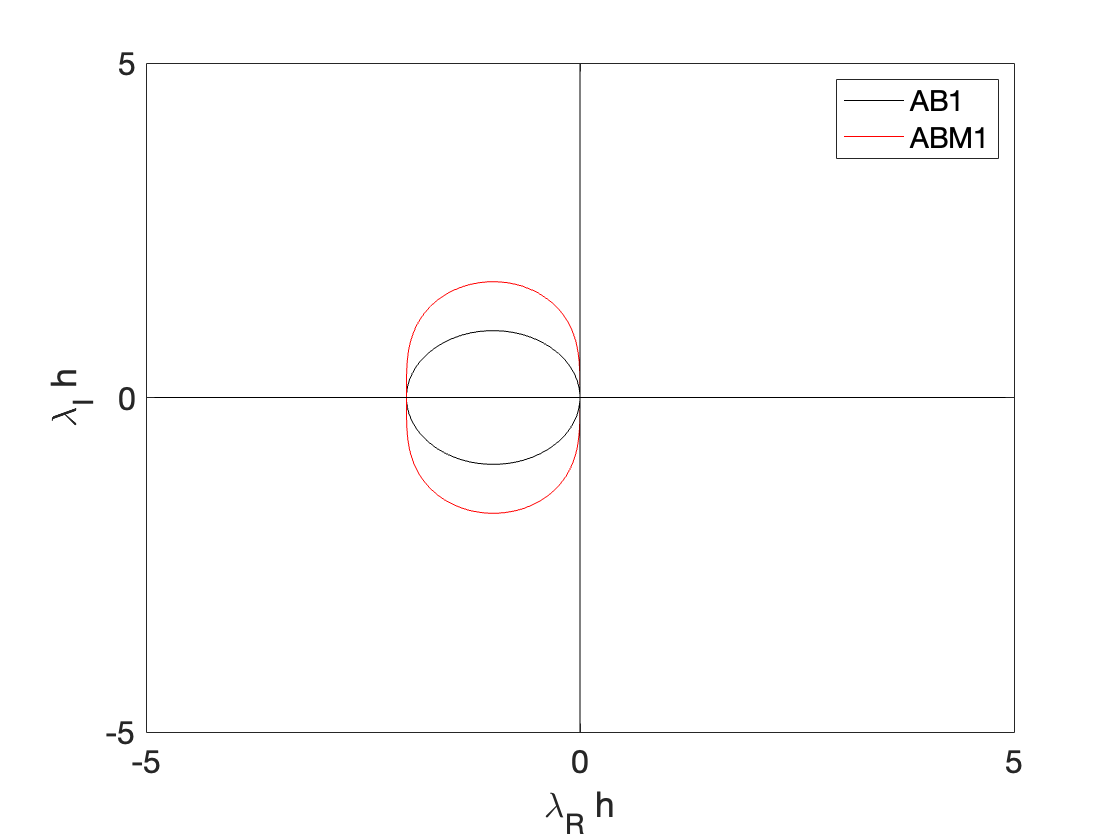
\includegraphics[width=0.5\textwidth]{p1_1.png}
  \caption{Linear stability diagram after the first corretor step. }
  \label{fig1_1}
\end{figure}

This is the RK2 Method. Comparing stability of those three methods, AM2>ABM1>AB1. 
\subsection{c}
For one corrector step, 
\begin{align*}
  k_1&=y_{n+1}=y_n+\lambda h y_n+\frac{(\lambda h)^2}{2}y_n\\
  \sigma_1&=1+\lambda h+\frac{(\lambda h)^2}{2}
\end{align*}

For two corrector steps, 
\begin{align*}
  k_2=y_{n+1}&=y_n+\frac{h}{2}\left(k_1^{'}+y_n^{'}\right)\\
  &=y_n+\frac{h}{2}\left(\lambda y_n+\lambda^2hy_n+\frac{\lambda^3h^2}{2}y_n+\lambda y_n\right)\\
  &=y_n+\lambda h y_n+\frac{\lambda^2 h^2}{2}y_n+\frac{\lambda^3 h^3}{4}\\
  \sigma_2&=1+\lambda h+\frac{(\lambda h)^2}{2}+\frac{(\lambda h)^3}{4}
\end{align*}

With similar derivation process,  
\begin{align*}
  \sigma_3&=1+\lambda h+\frac{(\lambda h)^2}{2}+\frac{(\lambda h)^3}{4}+\frac{(\lambda h)^4}{8}\\
  \sigma_4&=1+\lambda h+\frac{(\lambda h)^2}{2}+\frac{(\lambda h)^3}{4}+\frac{(\lambda h)^4}{8}+\frac{(\lambda h)^5}{16}\\
  \sigma_n&=1+\sum_{i=1}^{n} \frac{(\lambda h)^i}{2^{i-1}}\approx 1+\frac{\lambda h\left(1-\left(\frac{\lambda h}{2}\right)^n\right)}{1-\frac{\lambda h}{2}}\approx 1+\frac{\lambda h(1-0)}{1-\frac{\lambda h}{2}}\\
  &=\frac{1+\frac{\lambda h}{2}}{1-\frac{\lambda h}{2}}
\end{align*}

The stability diagram after 2,3,4,5,6,7 corrector steops are shown in Fig.~\ref{fig1_2}. The real-axis stability keep $[-2,0]$.
\begin{figure}[h]
  \centering
  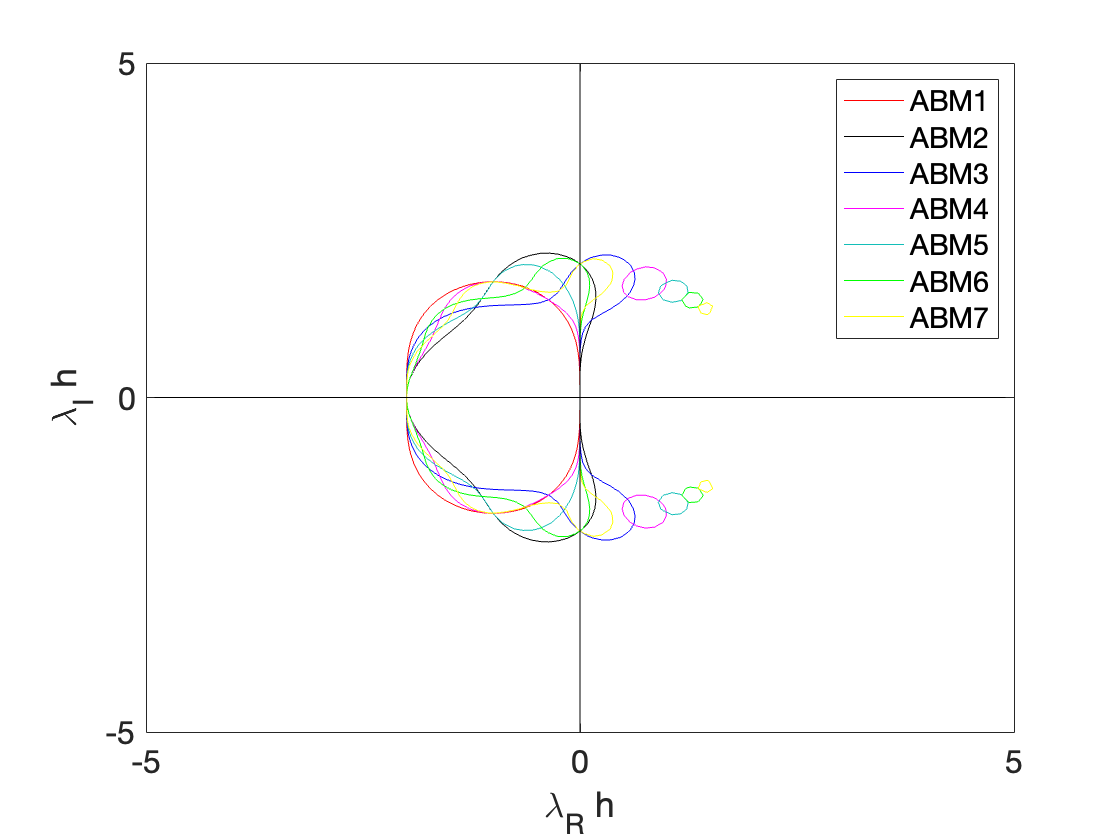
\includegraphics[width=0.5\textwidth]{p1_2.png}
  \caption{Linear stability diagram after 2,3,4,5,6,7 corretor steps. }
  \label{fig1_2}
\end{figure}
\subsection{d}
From the above plot and equations, when increasing corrector steps, the semi-implicit scheme might converge to the implicit scheme, e.g. AM2. 
\section{Haarmonically Forced Undamped Oscillator}
\subsection{a}
\begin{align*}
  \theta_{n+1} &= \theta_n+h\lambda_n\\
  \lambda_{n+1} &= \lambda_n -h \sin \theta_n - \frac{h^2}{2}\lambda_n \cos\theta_n +...\\
  \lambda_n-h\sin \theta_{n+1} &= \lambda_n-h\left(\sin \theta_n + h\lambda_n \cos \theta_n-\frac{h^2\lambda_n^2}{2}\sin \theta_n+...\right)\\
  &=\lambda_n-h\sin \theta_n - h^2\lambda_n \cos \theta_n+...
\end{align*}

So the order of accuracy of sympletic Euler method is $O(h^2)$. 
\subsection{b}
\begin{align*}
  \theta_{n+1} &= \theta_n+h\lambda_n\\
  \sin \theta_{n+1} &= \sin \theta_n + h\lambda_n \cos \theta_n-\frac{h^2\lambda_n^2}{2}\sin \theta_n+...\\
  |J|&=\begin{vmatrix}
    1&h\\-h(\cos \theta_n - h\lambda_n \sin \theta_n+...)&1-h(h\cos \theta_n-h^2\lambda_n\sin \theta_n+...)
  \end{vmatrix}\\
  &\approx 1-(h^2\cos \theta_n-h^3\lambda_n\sin \theta_n)+(h^2\cos \theta_n-h^2\lambda_n \sin \theta_n)+...\\
  &=1
\end{align*}

So the sympletic Euler method conserves the Hamiltonian. 
\subsection{c}
\begin{align*}
  x^{''}+\omega_n^2x&=\frac{F}{m}\cos \omega t\\
  x^{''}+25x&=\cos 0.1 t\\
  \Rightarrow x^{'}&=v\\
  v^{'}&=-25x+\cos 0.1t\\
  x(0)&=0\\
  x^{'}(0)&=v(0)=0
\end{align*}

For Forward Euler, 
\begin{align*}
  x_{n+1}&=x_n+hv_n\\
  v_{n+1}&=v_n-25hx_n+h\cos 0.1t\\
  \begin{vmatrix}
    x_{n+1}\\v_{n+1}
  \end{vmatrix}&=\begin{vmatrix}
    1&h\\-25h&1
  \end{vmatrix}\begin{vmatrix}
    x_n\\v_n
  \end{vmatrix}+\begin{vmatrix}
    0\\h\cos 0.1t
  \end{vmatrix}
\end{align*}
\subsection{d}
For Symplectic Euler,
\begin{align*}
  x_{n+1}&=x_n+hv_n\\
  v_{n+1}&=v_n-25hx_{n+1}+h\cos 0.1t\\
  v_{n+1}+25hx_n&=v_n+h\cos 0.1t\\
  \begin{vmatrix}
    1&0\\25h&1
  \end{vmatrix}
  \begin{vmatrix}
    x_{n+1}\\v_{n+1}
  \end{vmatrix}&=\begin{vmatrix}
    1&h\\0&1
  \end{vmatrix}\begin{vmatrix}
    x_n\\v_n
  \end{vmatrix}+\begin{vmatrix}
    0\\h\cos 0.1t
  \end{vmatrix}
\end{align*}
\subsection{e}
For RK4, 
\begin{align*}
  y_{n+1}&=y_n+\frac{1}{6}k_1+\frac{1}{3}(k_2+k_3)+\frac{1}{6}k_4\\
  k_1&=hf\left(t_n,y_n\right)\\
  k_2&=hf\left(t_n+\frac{1}{2}h,y_n+\frac{1}{2}k_1\right)\\
  k_3&=hf\left(t_n+\frac{1}{2}h,y_n+\frac{1}{2}k_2\right)\\
  k_4&=hf\left(t_n+h,y_n+k_3\right)
\end{align*}

From the equation $x^{''}+25x=\cos 0.1t$, $\omega_0=5$ is much large, so the main amplitude of $x$ should vibrate with much lower frequency. 
And $\omega=0.1$, so besides the lower vibration of amplitude, the $F$ adds a little fluctuation with much higher frequency on $x$. 

The general solution of such harmonically forced undamped oscillator is, 
\begin{equation*}
  x(t)=c_1\cos \omega_n t+c_2 \sin \omega_n t +\frac{F}{m(\omega_n^2-\omega^2)}\cos \omega t
\end{equation*}

For that system, the solution is, 
\begin{align*}
  x(t)&=-\frac{1}{50}\cos 5t +\frac{1}{50}\cos 0.1t\\
  v(t)&=\frac{1}{10}\sin 5t - \frac{1}{500} \sin 5t
\end{align*}

So there are two vibrations with a lower frequency and a higher frequency in the system. 

\subsubsection{i}
Fig.~\ref{fig2_1} shows the $x-t$ diagram. The x amplitue of Forward Euler increased quickly while Symplectic Euler and RK4 do not have obvious 
increase of amplitude. But all the three amplitude are larger than the exact value. The results from Symplectic Euler is similar to RK4. 
\begin{figure}[h]
  \centering
  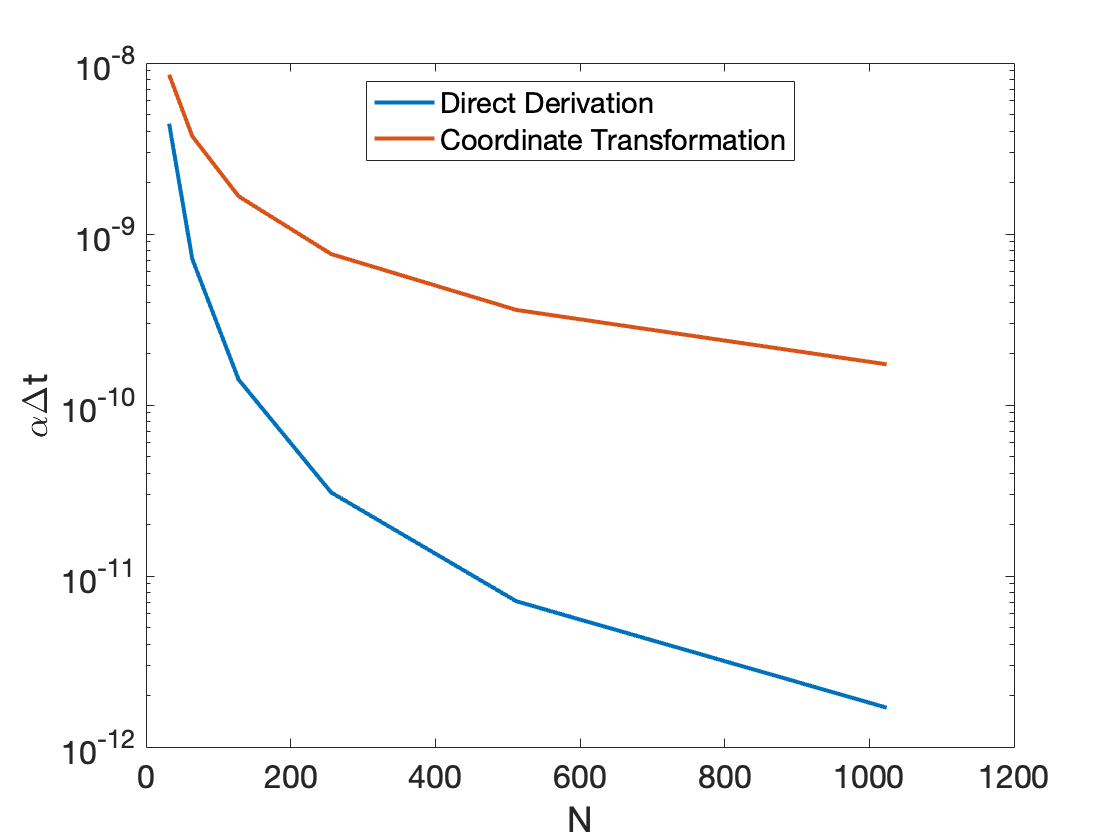
\includegraphics[width=0.5\textwidth]{p2_1.png}
  \caption{x(t)-t diagram. }
  \label{fig2_1}
\end{figure}

\subsubsection{ii}
Fig.~\ref{fig2_2} shows the $u-x$ diagram. The u amplitue vibrates along with the vibration of x amplication. Similarily, u amplitude of Forward Euler increased quickly while Symplectic Euler and RK4 do not have obvious increase of amplitude. But all the three amplitude are larger than the exact value. The results from Symplectic Euler is similar to RK4. 
\begin{figure}[h]
  \centering
  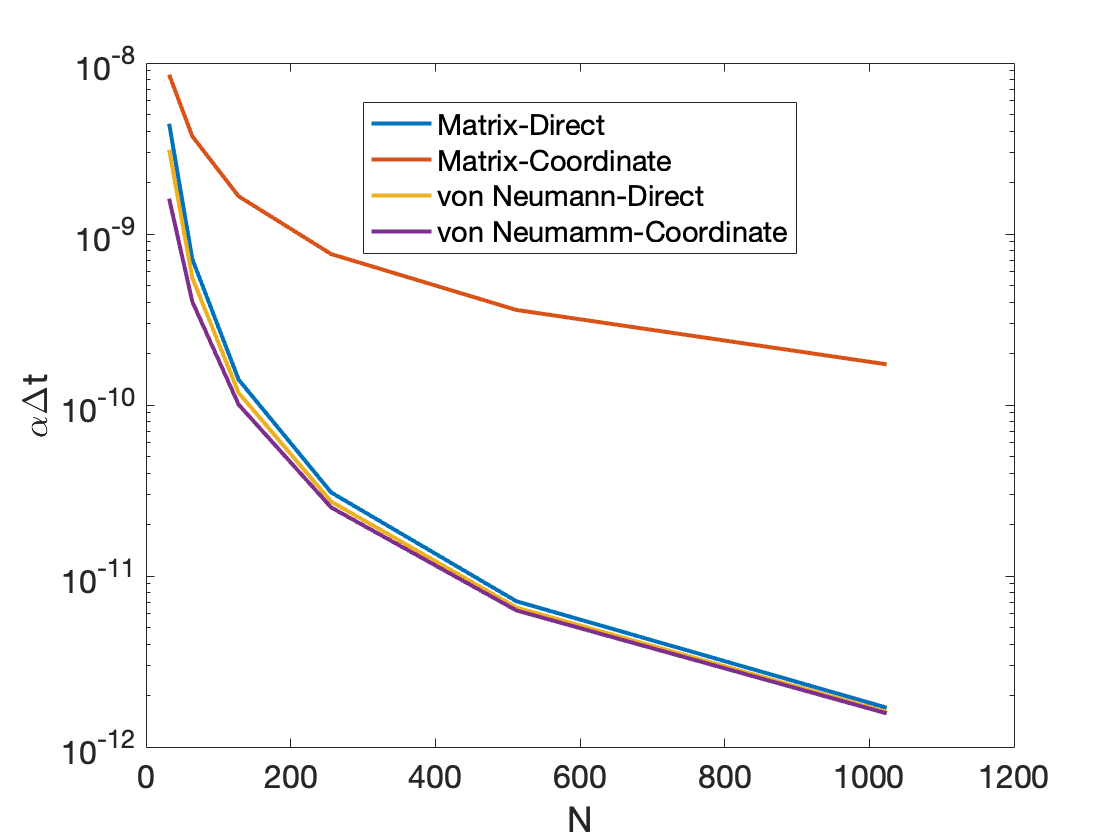
\includegraphics[width=0.5\textwidth]{p2_2.png}
  \caption{u(t)-x(t) diagram. }
  \label{fig2_2}
\end{figure}

\subsubsection{iii}
The error digram of the three methods is shown in Fig.~\ref{fig2_3}. The diagram of SE and RK4 only is Fig.~\ref{fig2_4}. So actually all the amplitude of the three methods will increase. Just the Forward Euler increases much quicker. The difference between SE and RK4 is small. But it still 
could be observed that RK2 is a bit more accurate than SE. 
\begin{figure}[h]
  \centering
  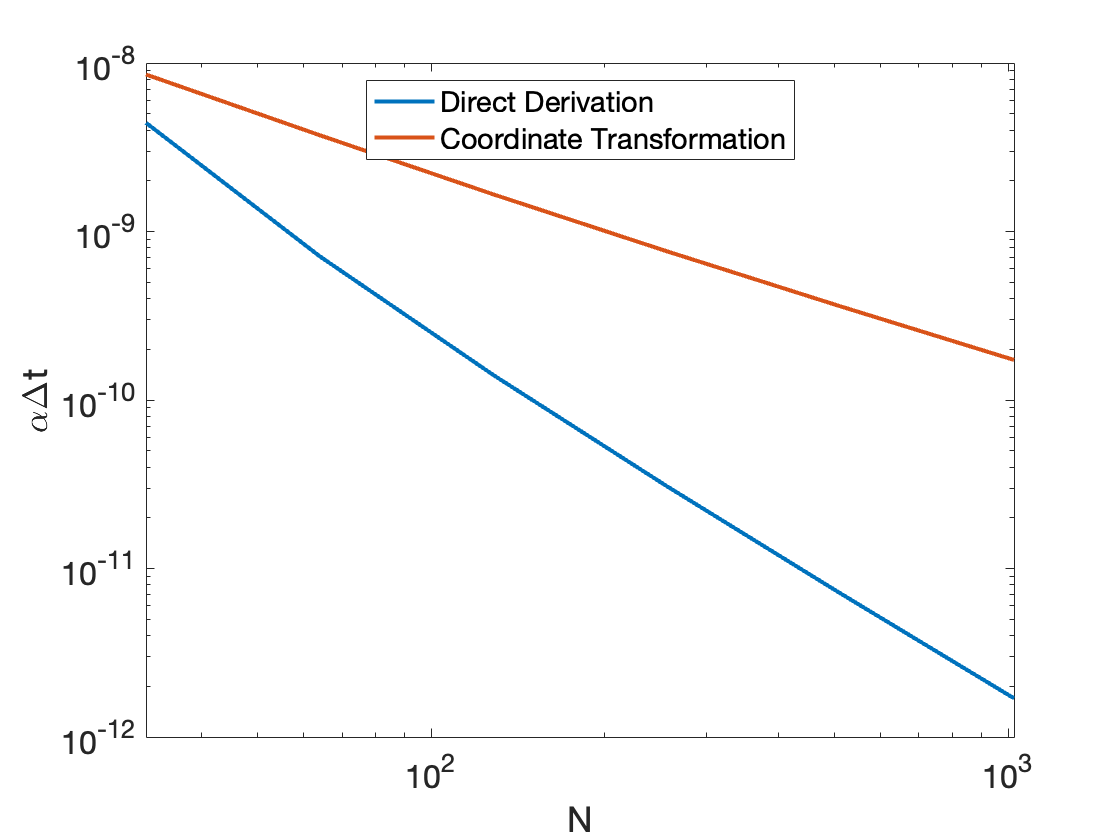
\includegraphics[width=0.5\textwidth]{p2_3.png}
  \caption{Error diagram of three methods. }
  \label{fig2_3}
\end{figure}

\begin{figure}[h]
  \centering
  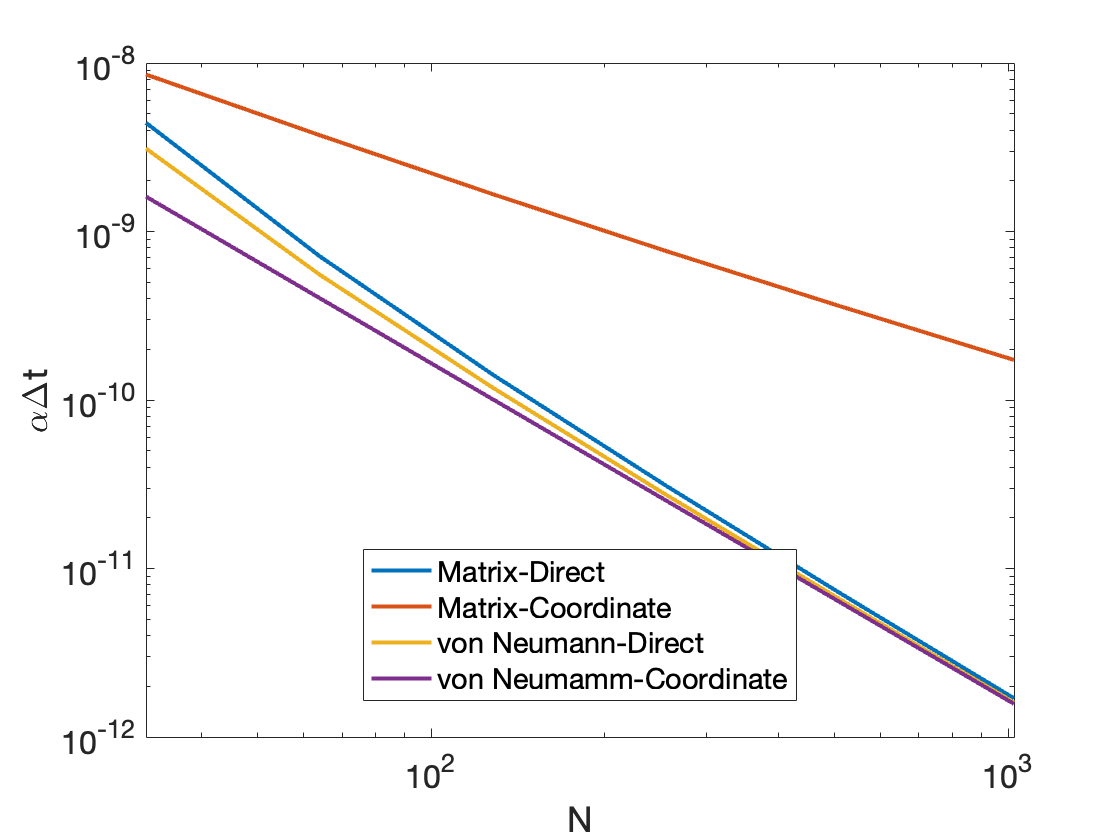
\includegraphics[width=0.5\textwidth]{p2_4.png}
  \caption{Error diagram of SE and RK4. }
  \label{fig2_4}
\end{figure}
\subsection{d}
The Fowrad Euler method is the most fast one, but the amplitude also blow up quickly. The RK4 is the most accurate one but expensive. And results from RK4 are still different from the exact value, just more stable. The Symplectic Euler method is cheaper than RK4 but the results is very similar so it is a middle one. With given amount of CPU time, the Symplectic Euler method will reach the highest degree of accuracy. None of them conserves energy. 
\section{Implicit and Explicit Analogs of Common Methods}
\subsection{a}
\begin{align*}
  y_{n+1}&=y_n+\frac{1}{2}k_1+\frac{1}{2}k_2\\
  k_1&=hf\left(t_n+\left(\frac{1}{2}-\frac{\sqrt{3}}{6}\right)h,y_n+\frac{1}{4}k_1+\left(\frac{1}{4}-\frac{\sqrt{3}}{6}\right)k_2\right)\\
  k_2&=hf\left(t_n+\left(\frac{1}{2}+\frac{\sqrt{3}}{6}\right)h,y_n+\frac{1}{4}k_2+\left(\frac{1}{4}+\frac{\sqrt{3}}{6}\right)k_1\right)
\end{align*}

With expansion of $k_1, k_2$ about $y_n$, 
\begin{align*}
  \left(1-\frac{\lambda h}{4}\right)k_1-\left(\frac{1}{4}-\frac{\sqrt{3}}{6}\right)\lambda hk_2&=hf\\
  \left(1-\frac{\lambda h}{4}\right)k_2-\left(\frac{1}{4}+\frac{\sqrt{3}}{6}\right)\lambda hk_1&=hf\\
  \Rightarrow k_1&=\frac{hf(1-\frac{\sqrt{3}}{6}\lambda h)}{1-\frac{\lambda h}{2}-\frac{1}{12}\lambda^2h^2}\\
  k_2&=\frac{hf(1+\frac{\sqrt{3}}{6}\lambda h)}{1-\frac{\lambda h}{2}-\frac{1}{12}\lambda^2h^2}\\
  y_{n+1}&=y_n\left(\frac{1+\frac{\lambda h}{2}-\frac{1}{12}\lambda^2 h^2}{1-\frac{\lambda h}{2}-\frac{1}{12}\lambda^2 h^2}\right)\\
  \sigma &=\frac{1+\frac{\lambda h}{2}-\frac{1}{12}\lambda^2 h^2}{1-\frac{\lambda h}{2}-\frac{1}{12}\lambda^2 h^2}
\end{align*}

The stability of IRK2, shown in Fig.~\ref{fig3_1}, is similar to AM2, when $\lambda_R>0$, it is unstable and when $\lambda_R<0$, it is unconditionally stable. 
\begin{figure}[h]
  \centering
  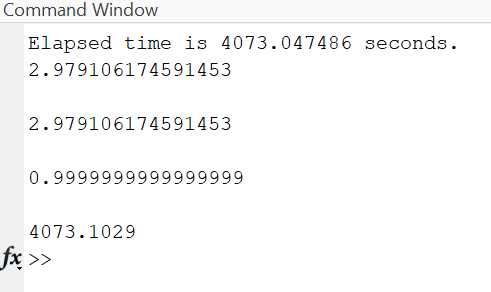
\includegraphics[width=0.5\textwidth]{p3_1.png}
  \caption{Linear stability diagram of IRK2. }
  \label{fig3_1}
\end{figure}

As an implicit multi-step method, even though this scheme has outstanding property of stability and accuracy. But at the same time, 
it is also reasonable that such scheme is very expensive. So in practice it is less likely to be used. 
\subsection{b}
For second-order, 
\begin{align*}
  y_{n+1}&=\beta f_n+\alpha_0 y_n \\
  \begin{vmatrix}
    1&0\\-h&1
  \end{vmatrix}\begin{vmatrix}
    \alpha_0\\\beta
  \end{vmatrix}&=\begin{vmatrix}
    1\\0
  \end{vmatrix}\\
  \Rightarrow y_{n+1}&=h f_n + y_{n}+O(h^2)\\
  \Rightarrow f_n &= \frac{y_{n+1}-y_{n}}{h}
\end{align*}

Obviously another name for the second-order method is first-order Adams-Bashforth method or Explicit Euler method. 

For third-order, 
\begin{align*}
  y_{n+1}&=\beta f_n+\alpha_0 y_n+\alpha_1 y_{n-1} \\
  \begin{vmatrix}
    1&1&0\\-h&-2h&1\\\frac{h^2}{2}&\frac{4h^2}{2}&-h
  \end{vmatrix}\begin{vmatrix}
    \alpha_0\\\alpha_1\\\beta
  \end{vmatrix}&=\begin{vmatrix}
    1\\0\\0
  \end{vmatrix}\\
  \Rightarrow y_{n+1}&=2h f_n +y_{n-1}+O(h^3)\\
  \Rightarrow f_n &= \frac{y_{n+1}-y_{n-1}}{2h}
\end{align*}

For second-order, 
\begin{align*}
  y_{n+1}&=h f_n +y_{n}+O(h^2)\\
  y_{n+1}-y_{n}&=\lambda h y_n\\
  \sigma^{n+1}-\sigma^{n}&=\lambda h \sigma^n\\
  \sigma&=\lambda h+1
\end{align*}

The linear stability diagram is shown in Fig.~\ref{fig3_2}, it is unconditionally unstable for purely imaginary $\lambda$. 
\begin{figure}[h]
  \centering
  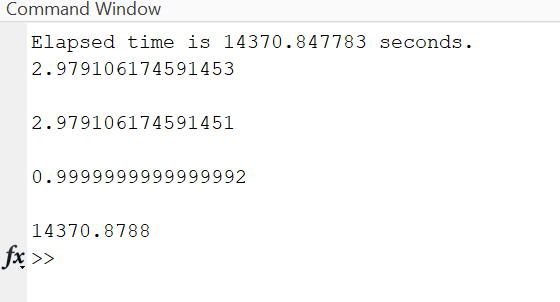
\includegraphics[width=0.5\textwidth]{p3_2.png}
  \caption{Linear stability diagram of EBDF2. }
  \label{fig3_2}
\end{figure}

For third-order, 
\begin{align*}
  y_{n+1}&=2h f_n +y_{n-1}+O(h^3)\\
  y_{n+1}-y_{n-1}&=2\lambda h y_n\\
  \sigma^{n+1}-\sigma^{n-1}&=2\lambda h \sigma^n\\
  \lambda h &=\frac{\sigma-\sigma^{-1}}{2}\\
  &=\frac{e^{i\theta}-e^{-i\theta}}{2}~for~\theta\in[0,2\pi]\\
  &=\frac{\cos\theta+i\sin\theta-\cos(-\theta)-i\sin(-\theta)}{2}\\
  &=i\sin\theta
\end{align*}

The linear stability diagram is shown in Fig.~\ref{fig3_3}, it is unconditionally stable for purely imaginary $\lambda h\in [-1,1]$. 
\begin{figure}[h]
  \centering
  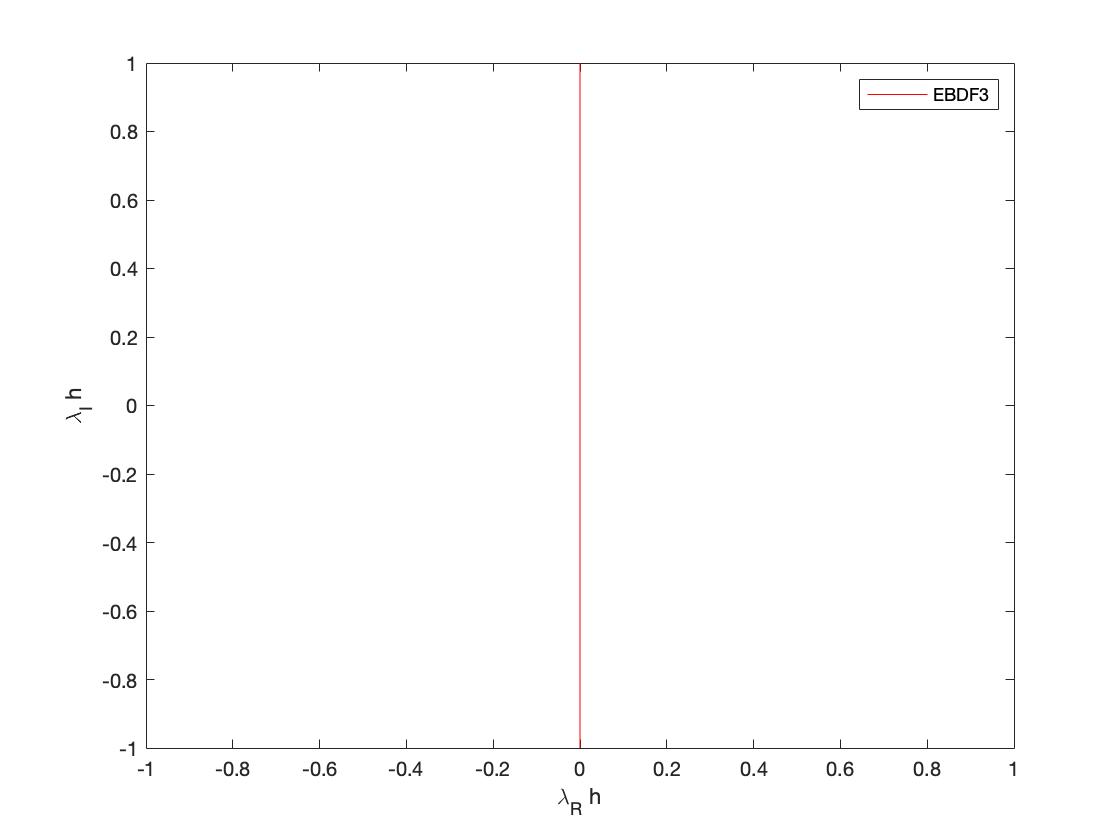
\includegraphics[width=0.5\textwidth]{p3_3.png}
  \caption{Linear stability diagram of EBDF3. }
  \label{fig3_3}
\end{figure}

So if the system has only imaginary $\lambda$, the third-order method is better under $h<\frac{1}{\lambda}$. If the system does not have 
only pure imaginary and $\lambda h$ locates within the circle, the second-order method could be used. 
\section{Stiff Systems of ODEs}
\subsection{a}
\begin{align*}
  J&=\begin{vmatrix}
    -k_{1f}X_{O}&0&k_{1b}X_{NO}&-k_{1f}X_{N^2}&k_{1b}X_{N}\\
    0&-k_{2f}X_{N}&-k_{2f}X_{O^2}&0&0\\
    k_{1f}X_{O}&-k_{2f}X_{N}&-k_{1b}X_{NO}-k_{2f}X_{O^2}&k_{1f}X_{N^2}&-k_{1b}X_{N}\\
    -k_{1f}X_{O}&k_{2f}X_{N}&k_{1b}X_{NO}+k_{2f}X_{O^2}&-k_{1f}X_{N^2}&k_{1b}X_{N}\\
    k_{1f}X_{O}&k_{2f}X_{N}&-k_{1b}X_{NO}+k_{2f}X_{O^2}&k_{1f}X_{N^2}&-k_{1b}X_{N}\end{vmatrix}\\
    &=\begin{vmatrix}
      -20&0&0&-1500&3e-14\\
      0&-0.2&-4.6&0&0\\
      20&-0.2&-4.6&1500&-3e-14\\
      -20&0.2&4.6&-1500&3e-14\\
      20&0.2&4.6&1500&-3e-14
  \end{vmatrix}\\
  \Rightarrow \lambda = \begin{vmatrix}
    -1.5245&0&-0.0003&0&0
  \end{vmatrix}\\
  \Rightarrow S&=\frac{\max |\lambda_i|}{\min |\lambda_i|}\gg 1
\end{align*}

The system is stiff. 
\subsection{b}
The results of three methods are shown in Fig.~\ref{fig4_1}-Fig.~\ref{fig4_5}. The AM and BDF need much less time steps to solve those ODEs and their 
results are also more stable so they are more suitable than RK4. The BDF is the cheapest one. Cheap but still good working, that is why I choose BDF over AM. 
\begin{figure}[h]
  \centering
  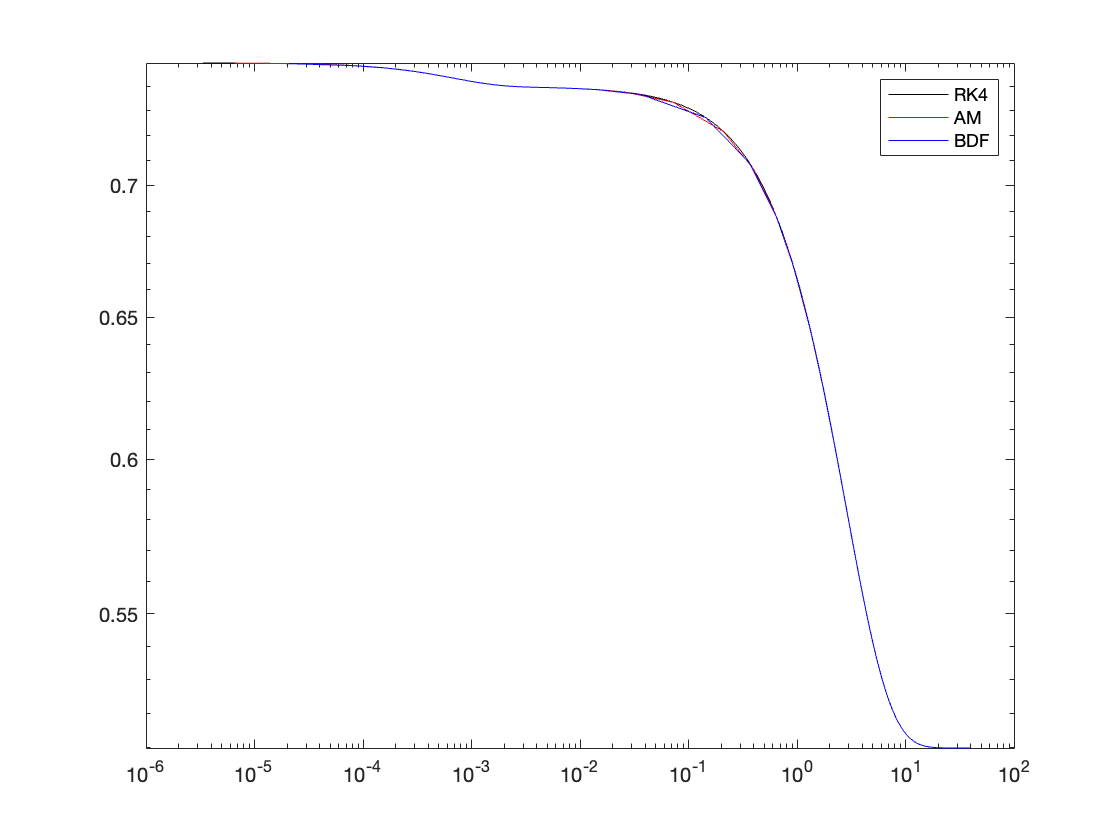
\includegraphics[width=0.5\textwidth]{p4_1.png}
  \caption{log(N2)-log(t). }
  \label{fig4_1}
\end{figure}

\begin{figure}[h]
  \centering
  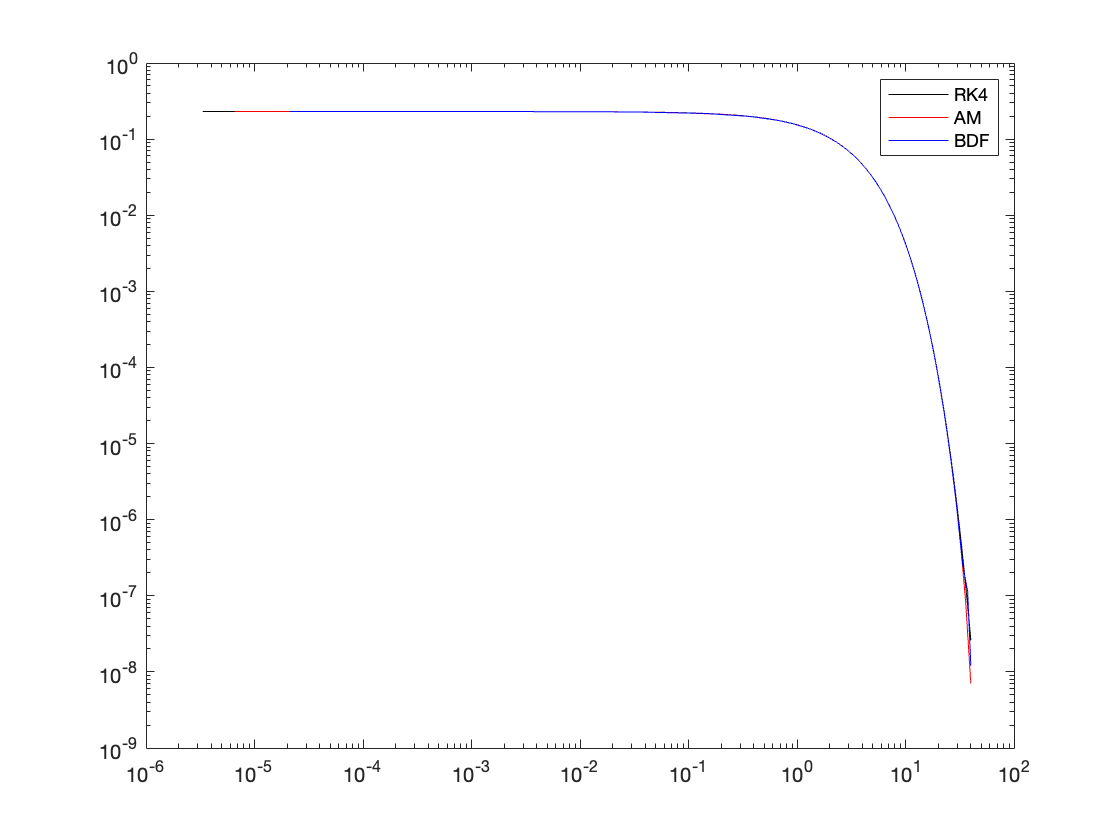
\includegraphics[width=0.5\textwidth]{p4_2.png}
  \caption{log(O2)-log(t). }
  \label{fig4_2}
\end{figure}

\begin{figure}[h]
  \centering
  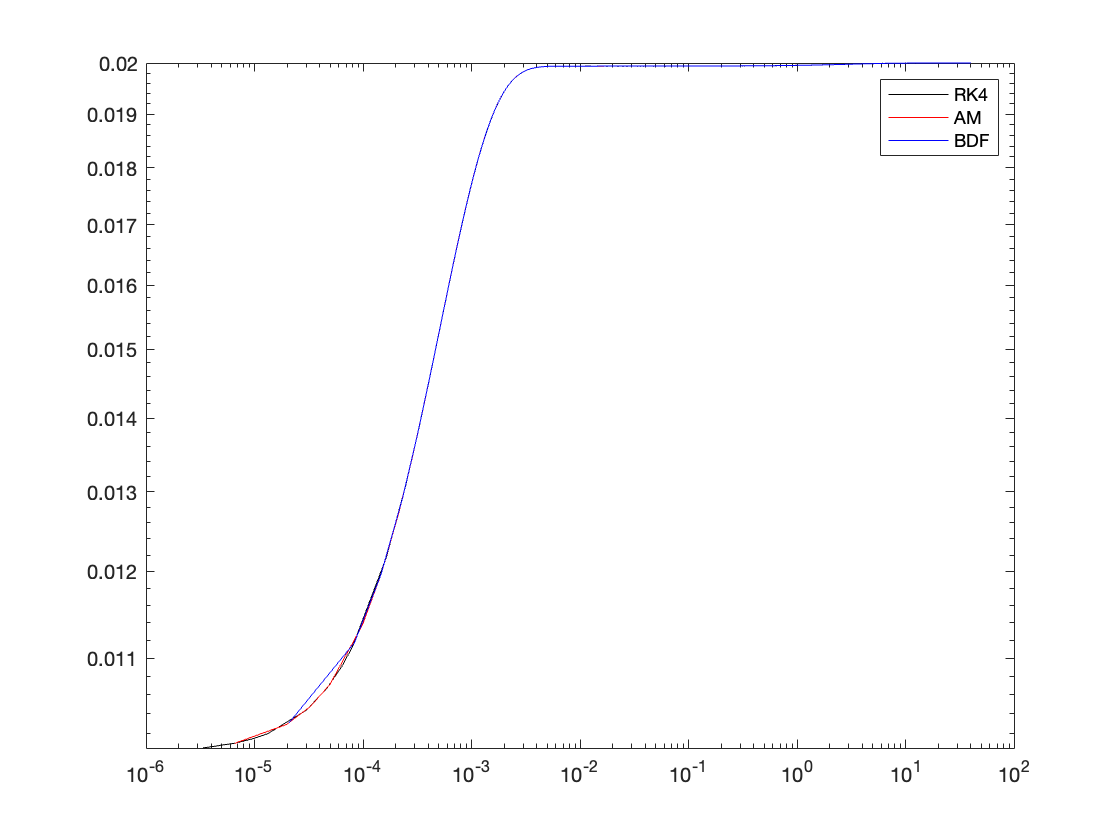
\includegraphics[width=0.5\textwidth]{p4_3.png}
  \caption{log(N)-log(t). }
  \label{fig4_3}
\end{figure}

\begin{figure}[h]
  \centering
  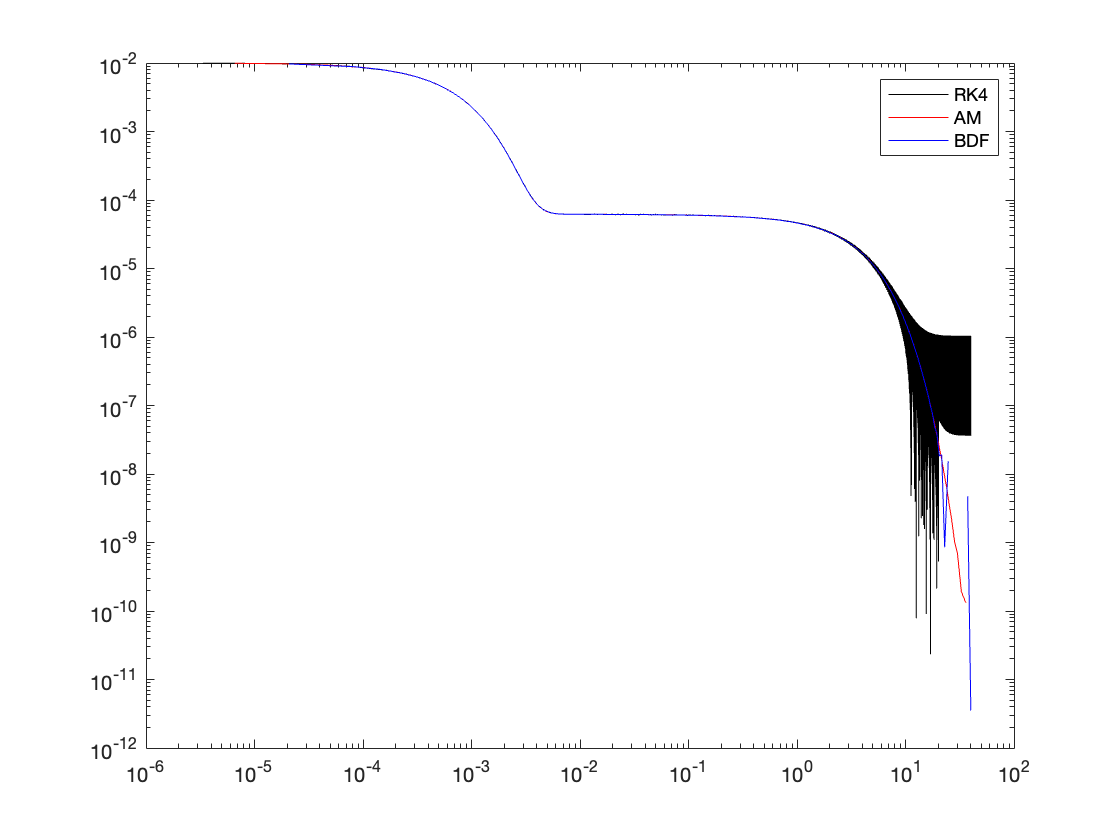
\includegraphics[width=0.5\textwidth]{p4_4.png}
  \caption{log(O)-log(t). }
  \label{fig4_4}
\end{figure}

\begin{figure}[h]
  \centering
  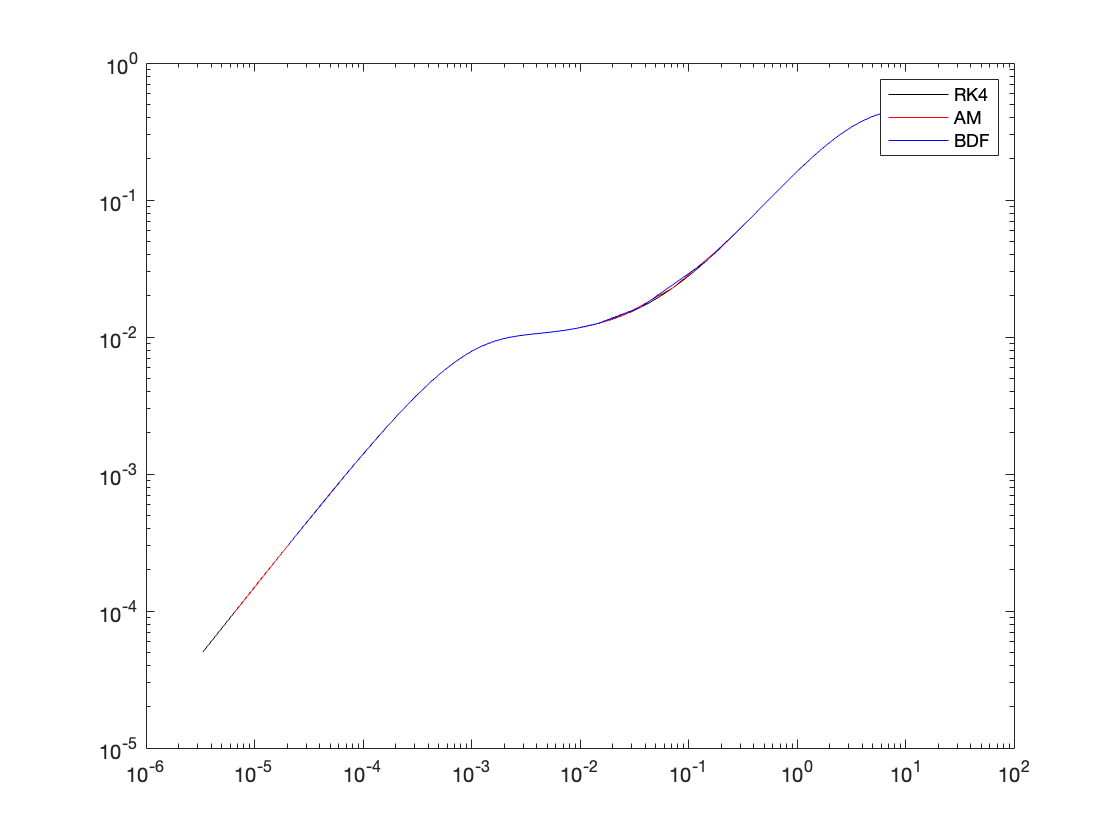
\includegraphics[width=0.5\textwidth]{p4_5.png}
  \caption{log(NO)-log(t). }
  \label{fig4_5}
\end{figure}
\end{document}